\begin{figure}
  \centering
  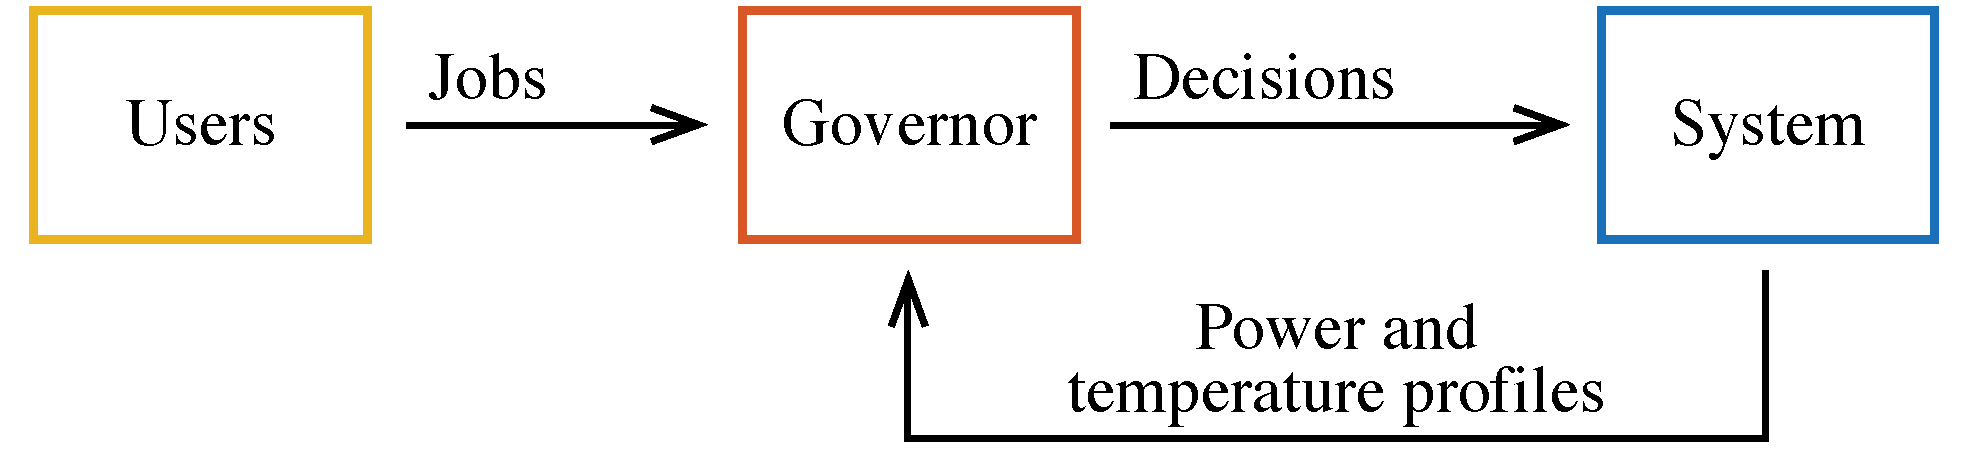
\includegraphics[width=1.0\columnwidth]{include/assets/figures/usage.pdf}
  \caption{A usage scheme with a feedback.}
  \flab{usage}
\end{figure}

Before concluding this paper, we would like to illustrate how one can go about
acquiring reference data and to discuss some common schemes of integrating the
methodology into the workflow of a research project.

Reference arrival data are based on a dataset published by Google \cite{google}.
The dataset contains usage data of a computer cluster over a month period,
namely, May 2011.

The workload patterns are obtained by simulating applications from two widely
used benchmark suites, namely, from \sc{PARSEC} \cite{bienia2011} and \sc{SPEC
CPU2006} \cite{cpu2006}.

A usage example with a feedback loop is given in \fref{usage}. Our methodology
revolves about the box in the middle and provides the boxes to the sides.
